\chapter[Anexos]{Anexos}
\label{chap:anexos}

	\section[Anexo A]{\emph{Anexo A - Cálculo do Dimensionamento de Condutores}}
	\label{sec:anexoA}

		\begin{figure}[!h]
			\centering
			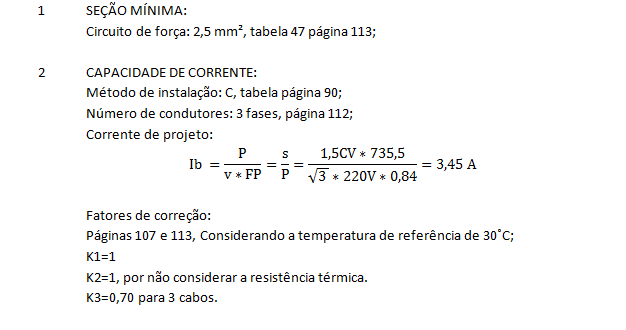
\includegraphics[scale=1]{AnexoA01.png}
			\caption{Anexo A - Parte I} 
			\label{AnexoA01}
		\end{figure}

		\newpage
		\begin{figure}[!h]
			\centering
			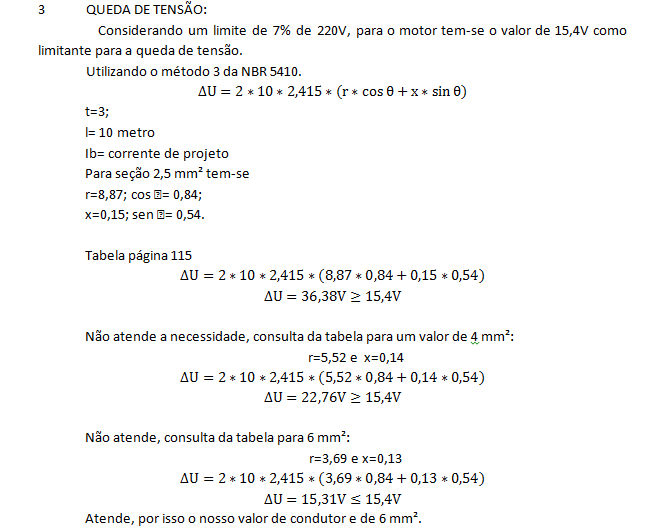
\includegraphics[scale=1]{AnexoA02.png}
			\caption{Anexo A - Parte II} 
			\label{AnexoA02}
		\end{figure}

		\newpage
		\begin{figure}[!h]
			\centering
			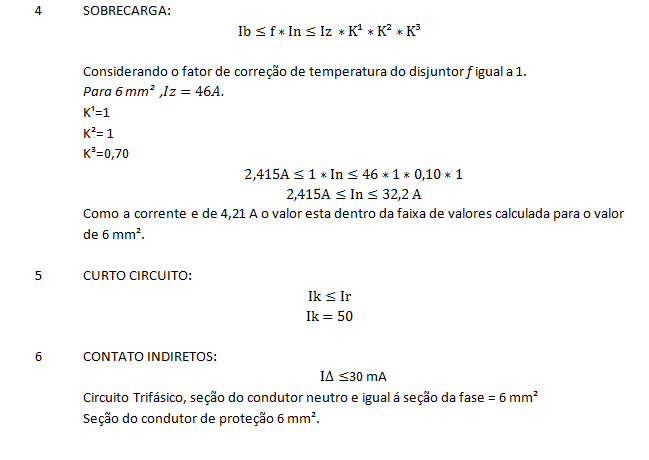
\includegraphics[scale=1]{AnexoA03.png}
			\caption{Anexo A - Parte III} 
			\label{AnexoA03}
		\end{figure}

	\newpage
	\section[Anexo B]{\emph{Anexo B - Programação dos Parâmetros no Inversor de Frequência para Variação das Velociades pelas Chaves Seletoras}}
	\label{sec:anexoB}

		O inversor foi programado para os seguintes parâmetros:

		\begin{itemize}
			\item Parâmetro P000 com o valor 5, liberando a programação do inversor;
			\item Parâmetro P204 com o valor 5, carregando as configurações de fábrica do inversor com dos equipamentos conectados de frequência de 60Hz;
			\item Novamente o parâmetro P000 com o valor 5;
			\item O parâmetro P220 com o valor 0;
			\item O parâmetro P221 com o valor 8;
			\item Parâmetro P223 com o valor 2;
			\item Parâmetro P224 com o valor 1, configurando assim a função multispeed;
			\item Para a configuração das velocidades, parâmetro P124 com o valor 200;
			\item Parâmetro P125 com o valor de 600;
			\item Parâmetro P126 com 1200;
			\item Parâmetro P127 com o valor de 1700;
		\end{itemize}

